\section{Lecture 14: The Gaseous Analytic Ring, Gaseous Real Vector Spaces, and the Tate Elliptic Curve}
\label{lec:14}

Scholze picks up the \emph{gaseous} analytic ring structure introduced at the end
of \cref{lec:12} and analyses it, using the general machinery Clausen developed on
Wednesday (\cref{lec:13}): the completion of a pre-analytic ring, and the
``killing an algebra object'' formula for the completion functor. The lecture has
three parts, matching the plan Scholze wrote down:
\begin{enumerate}
\item the \emph{gaseous base ring} --- a version of arithmetic Laurent series
$\ur A\subset\mathbb{Z}(\!(q)\!)$, cut out by a polynomial-growth condition on the
coefficients;
\item \emph{gaseous $\mathbb{R}$-vector spaces} --- the specialisation to the real
numbers, and its relation to the $\alpha$-liquid theory of \cref{lec:12};
\item a first pass at the \emph{construction of the Tate elliptic curve} over the
gaseous base ring, where one begins to need genuine analytic geometry (and the
language of analytic stacks, still to be introduced).
\end{enumerate}

Throughout, ``ring'' means commutative ring and everything lives in light
condensed abelian groups. We use freely the solid theory
(\cref{lec:5,lec:6}), the abstract notion of analytic ring and its completion
(\cref{lec:8,lec:13}), the compact projective generator
$P=\mathbb{Z}[\mathbb{N}\cup\{\infty\}]/[\infty]$ and its internal projectivity
(\cref{thm:3:three-properties,def:5:solid}), and the ``killing an algebra object''
construction of \cref{lec:13}. As in \cref{lec:12} the guiding example is the Tate
elliptic curve, and the goal is to pin down the \emph{smallest} analytic ring over
which it can be defined.

\subsection{The gaseous base ring}

\begin{remark}[Motivation and desiderata]
\label{rmk:14:motivation}
The motivation is to find a ``minimal'' analytic ring $(\ur A,\Mod_A)$ over which
the Tate elliptic curve $E_q$ can be defined. Two properties are needed of such a
ring, both with a transparent meaning in terms of the underlying condensed ring:
\begin{enumerate}
\item there is a topologically nilpotent unit $q\in\ur A$; and
\item if $P\otimes_{\mathbb{Z}}\ur A$ is the free $\ur A$-module on a null
sequence, then
\begin{equation}
\label{eq:14:desideratum}
1-q\cdot\mathrm{shift}\ \colon\ P\otimes_{\mathbb{Z}}\ur A\ \longrightarrow\ P\otimes_{\mathbb{Z}}\ur A
\end{equation}
is an isomorphism.
\end{enumerate}
Condition~(2) means that for a null sequence $(a_n)_n$ in $\ur A$ one can form the
sum $\sum_{n\ge 0} a_n q^n$: the inverse of $1-q\cdot\mathrm{shift}$ is
$1+q\cdot\mathrm{shift}+q^2\cdot\mathrm{shift}^2+\cdots$, and evaluating on the
zeroth coordinate produces exactly such a geometric series with null-sequence
coefficients. This is a genuine but \emph{weaker} completeness condition than
solidity: for solid modules one imposed the same isomorphism with $q=1$ (and did
not ask that $1$ be a topologically nilpotent unit), which forces summability of
\emph{all} null sequences, not only those weighted by powers of a topologically
nilpotent $q$ (\cref{def:5:solid}). Some completeness condition is essential ---
with none, one would work with all condensed modules and complete no infinite
series at all.
\end{remark}

Following the lightweight method of \cref{rmk:12:mindset-endomorphisms}, one turns
the two desiderata into an analytic ring by imposing that a natural endomorphism of
$P$ become an isomorphism. There is an evident initial (universal) example.

\begin{proposition}[The initial ring]
\label{prop:14:initial}
There is an initial analytic ring with the properties \eqref{eq:14:desideratum} of
\cref{rmk:14:motivation}. The same proof produces an initial \emph{animated} such
ring.
\end{proposition}

\begin{proof}[Construction]
Write
\begin{equation}
\label{eq:14:Zqhat}
\mathbb{Z}[\widehat{q}]\ :=\ \mathbb{Z}\bigl[q^{\mathbb{N}\cup\{\infty\}}\bigr]\big/(q^{\infty}=0),
\end{equation}
the free condensed ring on a topologically nilpotent element $q$; as a condensed
abelian group $\mathbb{Z}[\widehat{q}]=P$, the free module on the null sequence
$(q^n)_n$ (measures on $\mathbb{N}$, with the ring structure from addition, cf.\
\cref{rmk:7:P-ring}). Inverting $q$ gives the free condensed ring on a topologically
nilpotent \emph{unit}
\begin{equation}
\label{eq:14:A0}
\ur A_0\ :=\ \mathbb{Z}[\widehat{q}][\widehat{q}^{\,-1}].
\end{equation}
This is the underlying ring on which desideratum~(1) is tautological: a map
$\ur A_0\to{A'}^{\triangleright}$ is the same as a topologically nilpotent unit of ${A'}^{\triangleright}$. For
desideratum~(2), form $P\otimes_{\mathbb{Z}}\ur A_0$ with its endomorphism
$1-q\cdot\mathrm{shift}$ and declare
\begin{equation}
\label{eq:14:preanalytic-modules}
\Mod_A\ :=\ \Bigl\{\,M\in\Mod_{\ur A_0}\ \Big|\ 1-q\cdot\mathrm{shift}\ \text{is an isomorphism on}\ \iHom\bigl(P\otimes_{\mathbb{Z}}\ur A_0,\,M\bigr)\,\Bigr\}.
\end{equation}
Exactly as for solid modules (\cref{prop:5:solid-abelian}), the internal
projectivity of $P$ makes $\Mod_A\subseteq\Mod_{\ur A_0}$ closed under all the
operations required of an analytic ring, so $(\ur A_0,\Mod_A)$ is a
\emph{pre-analytic} ring in the sense of \cref{def:13:pre-analytic-ring}. It is not
analytic, because $\ur A_0\notin\Mod_A$: the base ring $\ur A_0$ is uncompleted.
Conditions~(1)$+$(2) on an analytic ring are precisely the datum of a map out of
$(\ur A_0,\Mod_A)$, so the completion of $(\ur A_0,\Mod_A)$ in the sense of
\cref{prop:13:completion} is the required initial analytic ring
$(\ur A,\Mod_A)$. The animated statement is proved the same way; it will turn out
below that the derived completion already lives in degree $0$, so the animated
initial object agrees with the classical one.
\end{proof}

We now compute this analytic ring $(\ur A,\Mod_A)=:A$.

\begin{theorem}[Structure of the gaseous base ring]
\label{thm:14:gaseous-base}
The initial analytic (animated) ring $A$ of \cref{prop:14:initial} is described as
follows, and in particular sits in degree $0$.
\begin{enumerate}
\item $\ur A$ and all free modules $\ur A[T]$, for $T\in\ProFin_{\mathbb{N}}(\mathrm{Fin})$,
sit in degree $0$ and are quasiseparated.
\item $\ur A$ is the subring of $\mathbb{Z}(\!(q)\!)$ of Laurent series with
polynomially bounded coefficients:
\begin{equation}
\label{eq:14:A-underlying}
\ur A(\ast)\ =\ \Bigl\{\,\textstyle\sum_{n\in\mathbb{Z}} a_n q^n\ \Big|\ a_n=0\ \text{for}\ n\ll 0,\ |a_n|\ \text{has at most polynomial growth}\,\Bigr\},
\end{equation}
and, as a light condensed ring,
\begin{equation}
\label{eq:14:A-condensed}
\ur A\ =\ \bigcup_{k>0,\ n>0}\ \prod_{m\ge -n}\Bigl(\mathbb{Z}\cap\bigl[-(m+n)^{k},\,(m+n)^{k}\bigr]\Bigr)\,q^{m}.
\end{equation}
\item For $S=\varprojlim_i S_i\in\ProFin_{\mathbb{N}}(\mathrm{Fin})$, the free
complete module is the space of $\mathbb{Z}((q))$-valued measures on $S$ with
polynomially bounded coefficients,
\begin{equation}
\label{eq:14:A-free}
A[S]\ \subseteq\ \mathbb{Z}(\!(q)\!)[S]^{\solid}\ =\ \Bigl(\varprojlim_i\mathbb{Z}[\widehat{q}][S_i]\Bigr)[\widehat{q}^{\,-1}]\ =\ \Mmeas\bigl(S,\mathbb{Z}(\!(q)\!)\bigr),
\end{equation}
namely
\begin{equation}
\label{eq:14:A-free-explicit}
\begin{aligned}
A[S]&=\Bigl\{\,\mu=\textstyle\sum_{m\in\mathbb{Z}}\mu_m q^m\ \Big|\
\mu_m\in\mathbb{Z}[S]\subseteq\mathbb{Z}[S]^{\solid},\\
&\hspace{12em}|\mu_m|\ \text{at most polynomial}\,\Bigr\}\\
&=\bigcup_{k>0,\ n>0}\ \varprojlim_i\ \prod_{m\ge -n}
\mathbb{Z}[S_i]_{\le (n+m)^{k}}\,q^{m}.
\end{aligned}
\end{equation}
\end{enumerate}
Here each $\mu_m$ is an \emph{honest} (finite) sum of Dirac measures --- for a fixed
power of $q$ no infinite sum is allowed --- and $\mathbb{Z}[S_i]_{\le N}$ denotes
sums of at most $N$ basis elements (see \cref{not:14:bounded}).
\end{theorem}

\begin{notation}[Bounded part of a free module]
\label{not:14:bounded}
For a finite set $I$ write
\begin{equation}
\label{eq:14:bounded}
\mathbb{Z}[I]_{\le n}\ :=\ \Bigl\{\,\textstyle\sum_{i\in I} a_i\,[i]\ \Big|\ \sum_i|a_i|\le n\,\Bigr\}\ \subseteq\ \mathbb{Z}[I],
\end{equation}
the (compact, light profinite) locus of measures of $\ell^1$-norm at most $n$.
\end{notation}

\begin{remark}[Where does polynomial growth come from?]
\label{rmk:14:surprise}
The polynomial-growth condition in \eqref{eq:14:A-underlying} is the surprising
output: in defining the gaseous structure one imposed only that $1-q\cdot\mathrm{shift}$
be invertible, with no growth condition visible anywhere. That this is what comes
out is exactly what happened to Clausen and Scholze when they first wrote down the
condition and computed. Note that polynomial growth is what makes $\ur A$ the
\emph{minimal} ring supporting $E_q$: the coefficients of the Tate-curve equation
have polynomial (not merely subexponential) growth (\cref{rmk:12:polynomial-growth}).
\end{remark}

\subsubsection*{Sketch of the computation}

\begin{proof}[Sketch of \cref{thm:14:gaseous-base}]
The computation runs through the completion formula from the end of
\cref{lec:13}. First rewrite the completeness condition
\eqref{eq:14:preanalytic-modules} as the vanishing of $\RHom$ out of a single
algebra object. Remembering the ring structure on $P=\mathbb{Z}[\widehat{q}]$, the
shift is multiplication by the nilpotent generator, so
\begin{equation}
\label{eq:14:B}
B\ :=\ \bigl(P\otimes_{\mathbb{Z}}\ur A_0\bigr)\big/(1-q\cdot\mathrm{shift})\ =\ \mathbb{Z}[\widehat{x},\widehat{q}][\widehat{q}^{\,-1}]\big/(1-qx)
\end{equation}
(writing $x$ for the generator of the source copy of $P$ and $q$ for the unit of
$\ur A_0$; multiplication by $x$ is the shift). It is a commutative ring, and
\begin{equation}
\label{eq:14:B-vanishing}
M\in\Mod_A\quad\Longleftrightarrow\quad \RHom_{\ur A_0}(B,M)=0,
\end{equation}
because this $\RHom$ is literally the cone of the map
$1-q\cdot\mathrm{shift}$ on $\iHom(P\otimes_{\mathbb{Z}}\ur A_0,M)$, and these
internal Homs sit in degree $0$ by internal projectivity of $P$. Moreover
$\RHom_{\ur A_0}(B,-)$ commutes with all colimits. Thus $B$ is an algebra object of
the ``killing'' type of \cref{def:13:killing}, and the derived completion in the
pre-analytic ring $(\ur A_0,\Mod_A)$ is given by the sequential-colimit formula of
\cref{constr:13:F,prop:13:left-adjoint}: with $I:=\mathrm{fib}(\mathbf 1\to B)$,
\begin{equation}
\label{eq:14:completion-formula}
M\ \longmapsto\ \operatorname*{colim}\Bigl(M\to\RHom(I,M)\to\RHom(I\otimes I,M)\to\cdots\Bigr),\qquad M\in D(\ur A_0).
\end{equation}

\emph{The key computation.} Everything reduces to computing internal Homs out of
$P$. One may proceed without inverting $q$ (and invert it at the end); doing so
replaces $\ur A_0$ by $P=\mathbb{Z}[\widehat q]$ and drops the terms with negative
powers of $q$. Writing $P=\mathbb{Z}[\widehat x]$ (free ring on a topologically
nilpotent $x$) and $y$ for the dual polynomial variable:

\begin{lemma}[Internal Homs out of $P$]
\label{lem:14:hom-P}
For $S=\varprojlim_i S_i\in\ProFin_{\mathbb{N}}(\mathrm{Fin})$,
\begin{equation}
\label{eq:14:hom-P-P}
\begin{aligned}
\iHom_{\mathbb{Z}}\bigl(P,\mathbb{Z}[\widehat{q}]\bigr)
&=\bigcup_{n>0}\varprojlim_m
\Bigl(\bigl(\mathbb{Z}[\widehat q]/\widehat q^{\,m}\bigr)_{\le n}[y]\Bigr),\\
\iHom_{\mathbb{Z}}\bigl(P,\mathbb{Z}[\widehat q][S]\bigr)
&=\bigcup_{n>0}\varprojlim_m
\Bigl(\bigl((\mathbb{Z}[\widehat q]/\widehat q^{\,m})[S_i]\bigr)_{\le n}[y]\Bigr).
\end{aligned}
\end{equation}
Equivalently these are the subspaces of ``bounded'' power series
\begin{equation}
\label{eq:14:hom-P-bdd}
\iHom_{\mathbb{Z}}\bigl(P,\mathbb{Z}(\!(q)\!)\bigr)=\mathbb{Z}[y][\![q]\!]^{\mathrm{bdd}}\subseteq\mathbb{Z}[y][\![q]\!],\qquad
\iHom_{\mathbb{Z}}\bigl(P,\mathbb{Z}[\widehat q][S]\bigr)=\mathbb{Z}[y][S][\![q]\!]^{\mathrm{bdd}}\subseteq\mathbb{Z}[y][S][\![q]\!],
\end{equation}
where $\mathrm{bdd}$ means the coefficient of each $y$-monomial satisfies the
$\le n$ boundedness property.
\end{lemma}

Since the free condensed abelian groups on light profinite sets are unions over $n$
of loci of norm $\le n$, this boundedness pulls through the internal Hom; the dual
variable $y$ appears because $\iHom$ out of the free ring on the nilpotent $x$ is
computed by polynomials in the dual variable.

\emph{From $\iHom$ to the Koszul complex.} With the boxed complex
$I=\mathrm{fib}(\mathbf 1\to B)$, formal manipulation of \eqref{eq:14:hom-P-bdd}
gives, in homological degrees $1$ and $0$,
\begin{equation}
\label{eq:14:RHom-I}
\RHom_{\mathbb{Z}[\widehat q]}\bigl(I,\,\mathbb{Z}[\widehat q]\bigr)\ =\ \Bigl[\ \mathbb{Z}[y][\![q]\!]^{\mathrm{bdd}}\ \xrightarrow{\ q-y\ }\ \mathbb{Z}[y][\![q]\!]^{\mathrm{bdd}}\ \Bigr],
\end{equation}
and for the $k$-fold tensor power the answer is a Koszul complex,
\begin{equation}
\label{eq:14:RHom-Ik}
\RHom_{\mathbb{Z}[\widehat q]}\bigl(I^{\otimes k},\,\mathbb{Z}[\widehat q]\bigr)\ =\ \mathbb{Z}[y_1,\dots,y_k][\![q]\!]^{\mathrm{bdd}}\big/^{\mathbb{L}}\bigl(q-y_1,\dots,q-y_k\bigr).
\end{equation}
It is crucial here that each individual term is computed by the full (derived)
Koszul complex, because there \emph{is} higher homology at each finite stage;
only the colimit is well behaved (nice, quasiseparated, in degree $0$). Feeding
\eqref{eq:14:RHom-Ik} into \eqref{eq:14:completion-formula} and doing the same with
$\mathbb{Z}[\widehat q][S]$ in place of $\mathbb{Z}[\widehat q]$ yields
\begin{equation}
\label{eq:14:A-colim}
\ur A\ =\ \operatorname*{colim}_k\ \mathbb{Z}[y_1,\dots,y_k][\![q]\!]^{\mathrm{bdd}}\big/^{\mathbb{L}}\bigl(q-y_1,\dots,q-y_k\bigr),
\end{equation}
and analogously for $A[S]$.

\emph{The growth condition.} Finally one analyses $H_0$ (or rather its
quasiseparated quotient): passing to $H_0$ means setting each $y_i=q$, i.e.\
computing the image of
\begin{equation}
\label{eq:14:image-question}
\mathbb{Z}[y_1,\dots,y_k][\![q]\!]^{\mathrm{bdd}}\ \longrightarrow\ \mathbb{Z}[\![q]\!],\qquad y_i\longmapsto q.
\end{equation}
For a fixed $n$, each occurrence of $q$ in a monomial can be routed either to a
$q$ or to one of $y_1,\dots,y_k$, and each $y_i$ may be used at most $n$ times; the
number of monomials of degree $<m$ in $k$ variables is $\binom{m+k-1}{k}$, so the
coefficient of $q^m$ in the image can be any integer in
\begin{equation}
\label{eq:14:coefficient-range}
\Bigl[\,-n\tbinom{m+k-1}{k},\ n\tbinom{m+k-1}{k}\,\Bigr],
\end{equation}
which grows in $m$ like a polynomial of degree $k$. Taking the union over $k$ and
$n$ produces exactly the polynomially-growing Laurent coefficients of
\eqref{eq:14:A-underlying}. Whenever a null sequence of coefficients ``grows and
decays normally'', the many available monomials let one split each summand into
bounded pieces; showing the Koszul complex collapses to degree $0$ amounts to
showing two such splittings differ by a bounded correction in the next term of the
complex, which needs to increase $k$ slightly but then works. The argument is of
the same flavour as the well-behavedness proofs in the liquid theory, but several
orders of magnitude easier.
\end{proof}

\begin{remark}[Individual terms versus the colimit]
\label{rmk:14:individual-terms}
As in the solid case, the individual terms of the colimit
\eqref{eq:14:completion-formula}--\eqref{eq:14:A-colim} are badly behaved --- spread
out, with higher homology, not quasiseparated. It is only the colimit that is nice.
Solidification itself is the degenerate case of this formula that one would obtain
by trying to use \eqref{eq:14:completion-formula} directly, and it is famously
confusing to run in that form; the gaseous case is where the colimit visibly does
something.
\end{remark}

\subsection{Gaseous real vector spaces}

The same lightweight recipe, applied with the topologically nilpotent unit
$\tfrac12\in\mathbb{R}$ in place of the formal $q$, produces an analytic ring
structure on $\mathbb{R}$. Throughout this subsection everything is light (the
qualifier is dropped).

\begin{definition}[Gaseous real vector space]
\label{def:14:gaseous-R}
A light condensed $\mathbb{R}$-vector space $V$ is \emph{gaseous} if
\begin{equation}
\label{eq:14:gaseous-R-def}
1-\tfrac12\cdot\mathrm{shift}\ \colon\ \iHom_{\mathbb{Z}}(P,V)\ \longrightarrow\ \iHom_{\mathbb{Z}}(P,V)
\end{equation}
is an isomorphism.
\end{definition}

\begin{remark}[Independence of the parameter]
\label{rmk:14:independent-half}
The condition \eqref{eq:14:gaseous-R-def} is independent of the choice of
$\tfrac12\in(0,1)$: any real number in $(0,1)$ would do. Intuitively, making the
number smaller weakens the condition, because the series one is asked to sum decays
faster; but one may always split off finitely many leading terms and telescope, so
the class of complete modules does not change. (This is unlike the liquid case,
where the analogous exponent $\alpha$ genuinely matters.)
\end{remark}

\begin{remark}[Gaseous is the weakest condition]
\label{rmk:14:gaseous-weakest}
Every $\alpha$-liquid (or $p$-liquid) real vector space is gaseous. So gaseous
vector spaces form an extremely general class of condensed real vector spaces --- the
$\alpha=0$ regime of the spectrum \eqref{eq:12:spectrum-interval} --- yet still
workable for many purposes.
\end{remark}

The following proposition ties \cref{def:14:gaseous-R} back to the gaseous base ring
of \cref{thm:14:gaseous-base}: gaseous real vector spaces are the modules of the
analytic ring obtained from $A$ by specialising $q\mapsto\tfrac12$.

\begin{proposition}[Specialisation $q\mapsto\tfrac12$]
\label{prop:14:specialise}
Let $A_{\mathrm{gas},\mathbb{R}}$ denote the analytic ring of gaseous real vector
spaces (it is an analytic ring structure by internal projectivity of $P$, as
usual). It is obtained from the gaseous base ring $A$ of \cref{thm:14:gaseous-base}
by the map $1-q\cdot\mathrm{shift}\mapsto 1-\tfrac12\cdot\mathrm{shift}$, i.e.\ by
setting $q=\tfrac12$; the completed ring $\ur A\otimes q\!\mapsto\!\tfrac12$ is
exactly $\mathbb{R}$ (the polynomial-growth Laurent series, evaluated at
$q=\tfrac12$, converge to real numbers). Consequently the free gaseous real vector
space on a light profinite $S=\varprojlim_i S_i$ is
\begin{equation}
\label{eq:14:free-gaseous-R}
\mathbb{R}[S]^{\mathrm{gas}}\ =\ \bigcup_{k>0}\ \bigcup_{c>0}\ \varprojlim_i\ \Bigl\{\,\textstyle\sum_{s\in S_i} x_s\,[s]\in\mathbb{R}[S_i]\ \Big|\ \sum_{s} f_k(x_s)\le c\,\Bigr\},
\end{equation}
for the functions $f_k$ of \cref{def:14:fk}.
\end{proposition}

Because $q$ has become the constant $\tfrac12$, the polynomial-growth condition of
\eqref{eq:14:A-underlying} can no longer be read off directly on the coefficients;
rephrasing it on $\mathbb{R}$ produces the ``crazy'' description
\eqref{eq:14:free-gaseous-R}, governed by a sequence of gauge functions.

\begin{definition}[The gauge functions $f_k$]
\label{def:14:fk}
The $f_k\colon\mathbb{R}\to\mathbb{R}_{\ge0}$ are any increasing functions such that,
for $|x|$ small,
\begin{equation}
\label{eq:14:fk}
f_k(x)\ =\ \bigl|\log|x|\bigr|^{-k}.
\end{equation}
For the transition maps of \eqref{eq:14:free-gaseous-R} to be defined one wants
$f_k$ increasing and \emph{concave}, so that
\begin{equation}
\label{eq:14:fk-subadditive}
f_k(x+y)\ \le\ f_k(x)+f_k(y);
\end{equation}
only the behaviour near $0$ matters (in an admissible infinite sum almost all terms
are tiny), so away from $0$ one extends $f_k$ arbitrarily, e.g.\ linearly. The
function $|\log|x||^{-k}$ is itself increasing and concave near $0$ but eventually
misbehaves --- at $x=1$ it blows up --- which is why one only prescribes it near the
origin.
\end{definition}

\begin{remark}[Which sums can be formed: liquid versus gaseous]
\label{rmk:14:sums}
The gauge functions encode which infinite sums a complete module can evaluate.
\begin{itemize}
\item In the $\alpha$-liquid theory ($\alpha\in(0,1]$) one can form
$\sum_{n\ge 0} x_n$ precisely when the sequence is \emph{$\beta$-summable} for some
$\beta<\alpha$, i.e.\ $\exists\,\beta<\alpha$ with $\sum_n|x_n|^{\beta}<\infty$.
\item In the gaseous theory one can form $\sum_n x_n$ only when
\begin{equation}
\label{eq:14:gaseous-summable}
\exists\,k\ \text{with}\ \sum_n f_k(x_n)<\infty,
\end{equation}
which is equivalent (up to reordering) to \emph{quasi-exponential decay} of the
terms:
\begin{equation}
\label{eq:14:quasi-exponential}
\exists\,\varepsilon>0,\ \exists\,C>0\ \colon\quad |x_n|\ \le\ C\cdot\Bigl(\tfrac12\Bigr)^{n^{\varepsilon}}.
\end{equation}
\end{itemize}
The equivalence is a direct computation: substituting $|x_n|=(\tfrac12)^{n^{\varepsilon}}$
into \eqref{eq:14:fk} turns the logarithm into $n^{\varepsilon}$, so
$f_k(x_n)\sim n^{-\varepsilon k}$, which is summable once $\varepsilon k>1$. Thus the
gaseous condition is a much stronger constraint on the summable sequences than any
liquid one --- one must have (nearly) exponential decay, not just power-law decay.
\end{remark}

% board 25 @ 01:44:33 --- unit "balls" of the liquid gauge |x|^beta and the gaseous gauge f_k, both non-convex, hugging the axes
\begin{center}
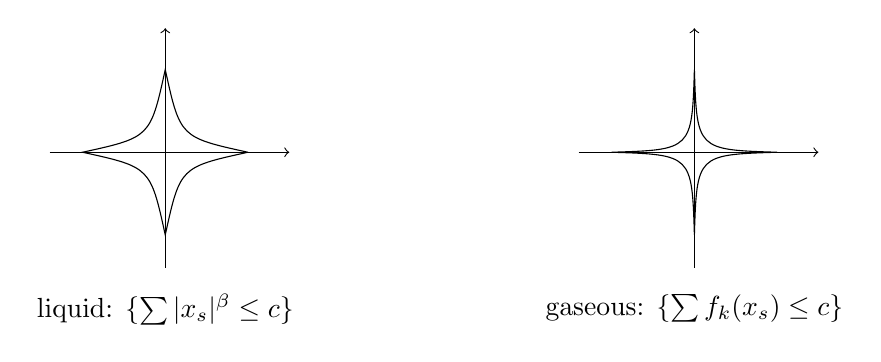
\begin{tikzpicture}[scale=1.05]
  % liquid: concave increasing gauge, star locus
  \begin{scope}[shift={(-3.2,0)}]
    \draw[->] (-1.4,0) -- (1.5,0);
    \draw[->] (0,-1.4) -- (0,1.5);
    \draw (1,0) .. controls (0.18,0.18) .. (0,1)
                .. controls (-0.18,0.18) .. (-1,0)
                .. controls (-0.18,-0.18) .. (0,-1)
                .. controls (0.18,-0.18) .. (1,0);
    \node[below] at (0,-1.6) {liquid: $\{\sum|x_s|^{\beta}\le c\}$};
  \end{scope}
  % gaseous: much sharper spikes along the axes
  \begin{scope}[shift={(3.2,0)}]
    \draw[->] (-1.4,0) -- (1.5,0);
    \draw[->] (0,-1.4) -- (0,1.5);
    \draw (1,0) .. controls (0.03,0.03) .. (0,1)
                .. controls (-0.03,0.03) .. (-1,0)
                .. controls (-0.03,-0.03) .. (0,-1)
                .. controls (0.03,-0.03) .. (1,0);
    \node[below] at (0,-1.6) {gaseous: $\{\sum f_k(x_s)\le c\}$};
  \end{scope}
\end{tikzpicture}
\end{center}

\begin{remark}[Gaseous suffices for complex geometry]
\label{rmk:14:complex-geometry}
The gaseous theory would serve just as well as the liquid theory for the analytic
geometry over $\mathbb{C}$ developed in Clausen--Scholze's notes on complex geometry
\cite{clausen2020analytic}: the only structural input there is that the algebras of
over-convergent holomorphic functions are nuclear, and this remains true in the
gaseous story. Indeed restriction of holomorphic functions from a disk to a smaller
one rescales the power-series coefficients by a fixed factor $<1$, so the transition
maps have exponential decay --- exactly the kind of decay
\eqref{eq:14:quasi-exponential} the gaseous theory is built to handle.
\end{remark}

\begin{remark}[Light versus all condensed sets]
\label{rmk:14:light-vs-all}
Asked whether non-light condensed sets are still used: originally extremally
disconnected sets were crucial, as they supplied enough projectives; for the present
theory one largely forgets the full category of condensed sets. It remains
occasionally convenient to have the ambient framework of all condensed sets --- light
objects embed into it, and one can test isomorphisms on extremally disconnected sets.
But for analytic geometry the light setting was chosen because of the internal
projectivity of $P$, used throughout. One can ask whether liquid and gaseous real
vector spaces can also be defined on \emph{all} condensed modules; probably yes, but
the arguments here use internal projectivity of $P$ and would need to be redone more
carefully.
\end{remark}

\subsection{Some gaseous geometry: the Tate elliptic curve}

Finally Scholze does a first piece of genuine analytic geometry over the gaseous base
ring, constructing the Tate elliptic curve. The construction uses the language of
analytic stacks --- the eventual subject of the course, still to be introduced --- but
the idea can already be stated.

\begin{remark}[Goal and idea]
\label{rmk:14:tate-goal}
The goal is to define the Tate elliptic curve $E_q$ over the gaseous base ring
$A=(\ur A,\Mod_A)$ of \cref{thm:14:gaseous-base}. The idea is that we have a fixed
topologically nilpotent unit $q$, and (as one always does with such a $q$) one
uses it to \emph{gauge} the size of any other function $f$: one asks
how powers $|f|^{\alpha}$ compare to powers $|q|^{\beta}$. Normalising $|q|=\tfrac12$
turns this into an ordinary real-valued absolute value.
\end{remark}

\begin{remark}[The gauge morphism]
\label{rmk:14:gauge-morphism}
The claim --- to be made precise once analytic stacks are available --- is that there
is a morphism of analytic stacks
\begin{equation}
\label{eq:14:gauge}
\mathbb{A}^1_A\ \xrightarrow{\ |T|\ }\ [0,\infty],
\end{equation}
where $T\in\ur A$ is the coordinate function; more precisely, on the projective line,
\begin{equation}
\label{eq:14:gauge-P1}
\mathbb{P}^1_A\ \xrightarrow{\ |T_1/T_2|\ }\ [0,\infty],\qquad [T_1:T_2]\ \longmapsto\ |T_1/T_2|,
\end{equation}
sending the two boundary points $0,\infty$ of $\mathbb{P}^1$ to the endpoints of the
closed interval. To define such a gauge for an arbitrary function it suffices to do it
for the universal one, the coordinate $T$ on $\mathbb{A}^1$.
\end{remark}

\begin{definition}[Analytic $\mathbb{G}_m$ and the Tate curve]
\label{def:14:tate-construction}
Define the analytic multiplicative group as the preimage of the open interval under
the gauge \eqref{eq:14:gauge-P1},
\begin{equation}
\label{eq:14:Gm-an}
{\Gm}^{\mathrm{an}}_{A}\ :=\ |T|^{-1}\bigl((0,\infty)\bigr)\ =\ \bigcup_{n}\ \bigl\{\,|q|^{n}\le |T|\le |q|^{-n}\,\bigr\},
\end{equation}
the rising union of annuli of all radii (this is what one starts from to define the
Tate curve). Multiplication by $q$ gives a free, totally discontinuous action on
${\Gm}^{\mathrm{an}}_{A}$, and the Tate elliptic curve is the quotient
\begin{equation}
\label{eq:14:Eq}
E_q\ :=\ {\Gm}^{\mathrm{an}}_{A}\big/q^{\mathbb{Z}}.
\end{equation}
\end{definition}

The gauge morphism is equivariant for multiplication by $q$ upstairs and by
$|q|=\tfrac12$ on $(0,\infty)$, so it descends to the quotients, giving a commuting
square:

% board 27 @ 01:41:39 --- Tate curve as quotient of the annulus G_m^an by q^Z, over the quotient of (0,infty) by (1/2)^Z = S^1
\[
\begin{tikzcd}[column sep=large, row sep=large]
{\Gm}^{\mathrm{an}}_{A} \arrow[r, "|T|"] \arrow[d, "/q^{\mathbb{Z}}"'] & (0,\infty) \arrow[d, "/(\frac12)^{\mathbb{Z}}"] \\
E_q \arrow[r] & (0,\infty)/(\tfrac12)^{\mathbb{Z}}=S^1
\end{tikzcd}
\]

\begin{proposition}[$E_q$ is a proper smooth curve]
\label{prop:14:Eq-proper-smooth}
The map ${\Gm}^{\mathrm{an}}_{A}\to(0,\infty)$ is proper (it is the restriction of the
proper $\mathbb{P}^1\to[0,\infty]$ over the open locus). Since $(0,\infty)\to(0,\infty)/(\tfrac12)^{\mathbb{Z}}=S^1$ is
proper and the $q^{\mathbb{Z}}$-action is free and totally discontinuous, the map
$E_q\to S^1$ is proper. Locally on $S^1$ the quotient map is an isomorphism onto an
open subset of $\mathbb{P}^1$, which is smooth; hence $E_q$ is a proper smooth curve
over $A$ --- the Tate elliptic curve.
\end{proposition}

\begin{remark}[Two roles of condensed mathematics; discrete rings suffice]
\label{rmk:14:two-roles}
The boundary points $0,\infty$ (and the interval $[0,\infty]$) are here regarded as
\emph{light condensed sets}, and there will be a functor from light condensed sets to
analytic stacks giving them an incarnation in this world. Consequently the theory of
analytic stacks will be tied to the condensed story in \emph{two} ways: first, the
analytic rings themselves are built on condensed sets (the role condensed mathematics
has played so far); and second, the geometric objects $[0,\infty]$, $S^1$, $\dots$
will themselves be realised through condensed sets. Notably, the realisation of $E_q$
as an analytic stack will use only \emph{discrete} rings --- no interesting condensed
structure at the ring level. This differs from the usual (adic-space) theory and will
be developed once the formalism of analytic stacks is set up.
\end{remark}
